The dc/dc converter used is the DCM Series 300V-24V VIA packaging, this converter was chosen, due to the efficiency, the input voltage range and output voltage, short-circuit protection, over voltage protection, under voltage protection, thermal protection and due to the reduced dimensions. In the Figure \ref{fig:DCpackaging} is shown the packaging of the DC/DC converter.
\begin{figure}[!htb]
	\centering
	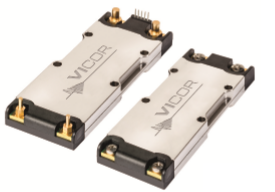
\includegraphics[width=0.5\linewidth]{Figures/DCM_packaging.PNG}
	\caption{DC/DC converter packaging.}
	\label{fig:DCpackaging}
\end{figure}\newline
In Table \ref{DCMSpecs} is shown the characteristics of the DCM converters.
\begin{table}[!htb]
\centering
\caption{DCM characteristics.}
\label{DCMSpecs}
\begin{tabular}{|l|l|lll}
\cline{1-2}
\textbf{Manufacturer}        & Vicor Power                                                                                                      &  &  &  \\ \cline{1-2}
\textbf{Model}               & DC/DC Converter DCM Series 300V-24V VIA packaging                                                                &  &  &  \\ \cline{1-2}
\textbf{Part number}         & DCM3714VD2H26F0C01                                                                                               &  &  &  \\ \cline{1-2}
\textbf{Nominal Power}       & 600 W                                                                                                            &  &  &  \\ \cline{1-2}
\textbf{Output current}      & 25 A                                                                                                             &  &  &  \\ \cline{1-2}
\textbf{Power density}       & 309 W/in3                                                                                                        &  &  &  \\ \cline{1-2}
\textbf{Protection}          & \begin{tabular}[c]{@{}l@{}}Safety Extra Low Voltage (SELV)\\   Short circuit and thermal protection\end{tabular} &  &  &  \\ \cline{1-2}
\textbf{Input voltage range} & 200-420 V DC                                                                                                     &  &  &  \\ \cline{1-2}
\textbf{Output voltage}      & 24 V DC                                                                                                          &  &  &  \\ \cline{1-2}
\textbf{Dimension}           & \begin{tabular}[c]{@{}l@{}}3.750” x\\   1.400” x 0.370” (95.13 mm x 35.5 mm x 9.30 mm)\end{tabular}              &  &  &  \\ \cline{1-2}
\end{tabular}
\end{table}